%!TEX root = ../../main.tex


\begin{figure}[!htb]
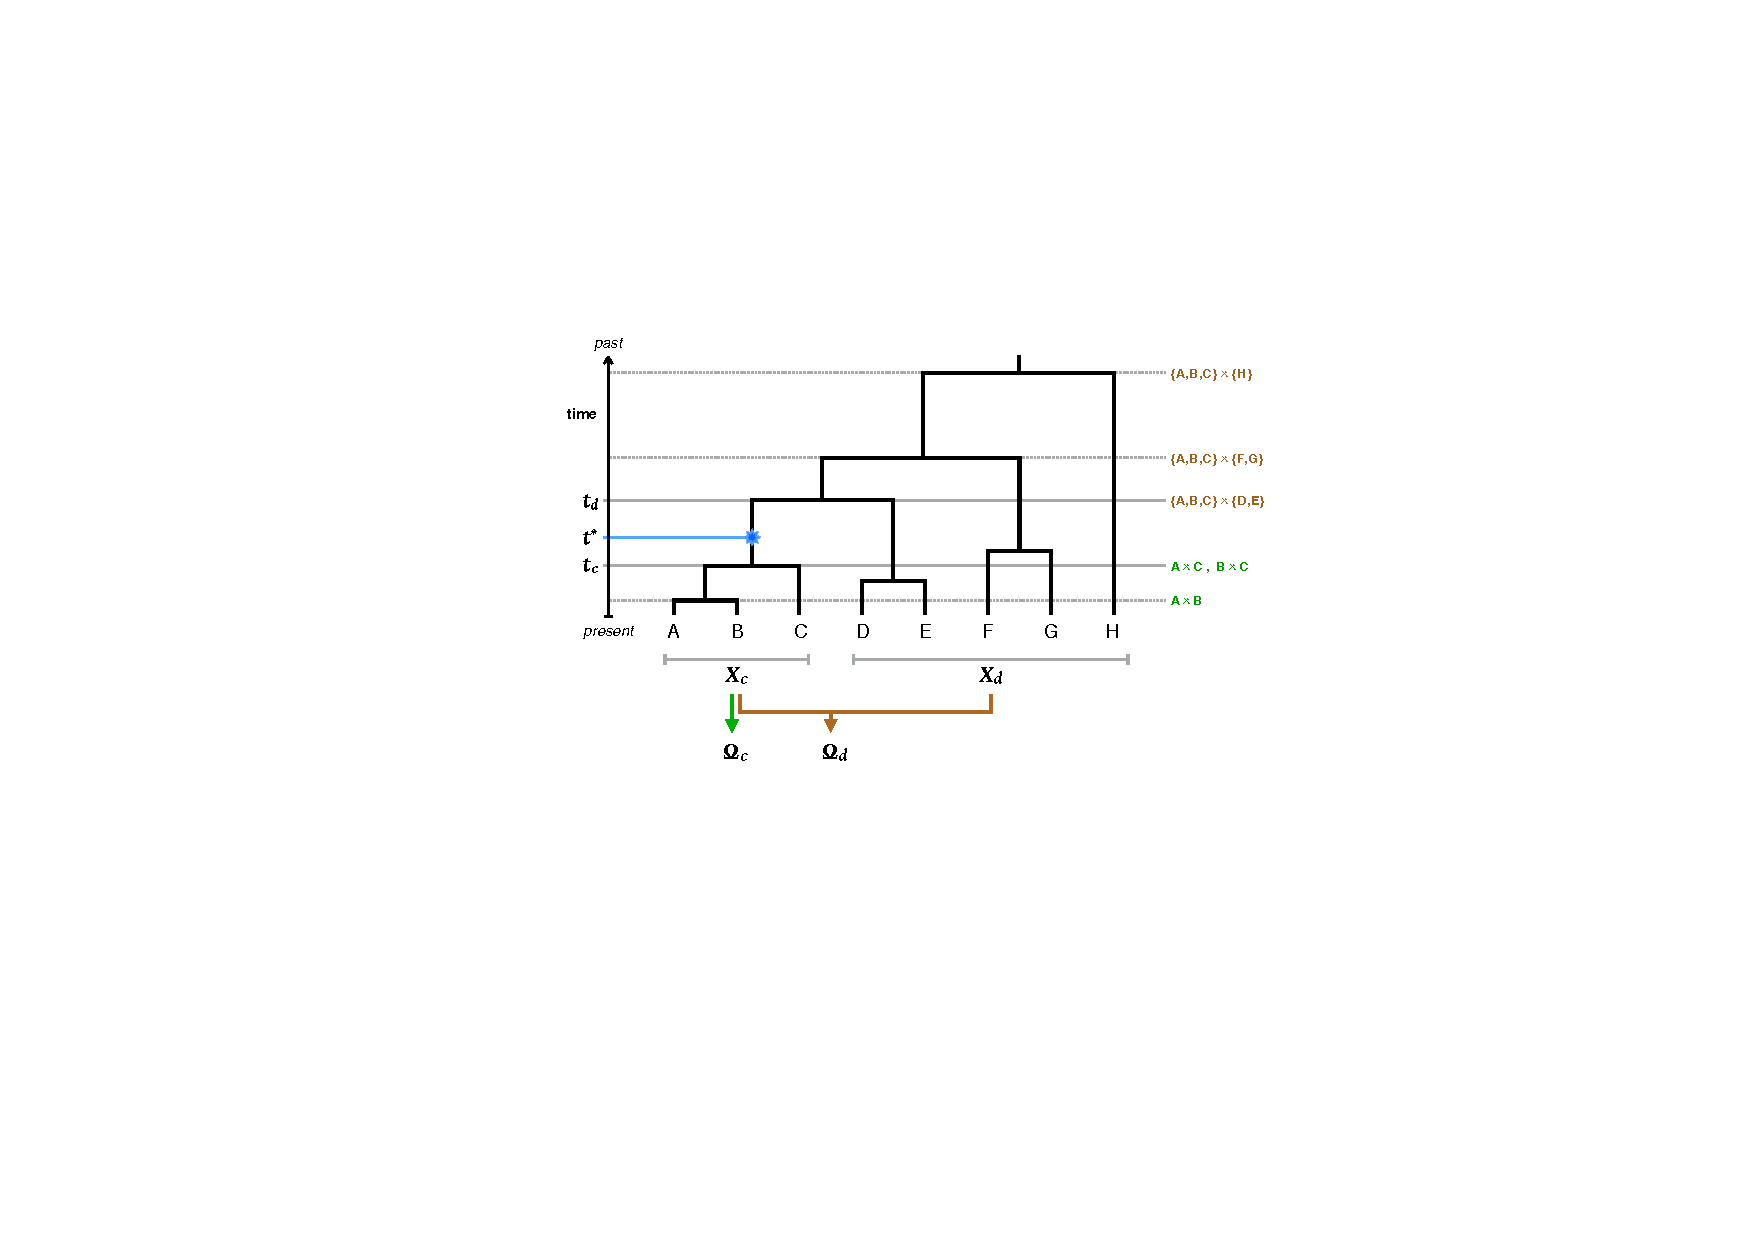
\includegraphics[width=\textwidth]{./img/ch5/info_age}
\Caption{Allele age in relation to concordant and discordant pairs}%
{The genealogy of a sample of \n{8} haplotypes is shown of which A, B, and C share a focal allele that derived from a mutation event as indicated in the tree (\emph{star}).
These chromosomes constitute the set of \emph{carriers}, denoted by $X_c$, which are distinguished from the set of \emph{non-carriers}, denoted by $X_d$.
Horizontal lines indicate the time of each coalescent event in the history of the sample within the local genealogy.
The time of the focal mutation event is denoted by ${t^\ast}$; the \n{2} coalescent events at time $t_c$ and $t_d$ define the length of the branch on which the focal mutation event occurred.
In particular, $t_c$ and $t_d$ correspond to the time until all haplotypes in $X_c$ have coalesced and the time at which the derived lineage joins the ancestral lineage of the most closely related haplotype in $X_d$, respectively.}%
{fig:info_age}
\end{figure}


% {\scriptsize \texthv{\textbf{(b)}}} \\
% \vspace{-30pt}
% \begin{center}
% \begin{tikzpicture}[-,auto,thick,
% txt/.style={font=\helvet\footnotesize,text width=4cm},
% lab/.style={font=\helvet\footnotesize,rectangle,draw=white,minimum size=0.2cm},
% sub/.style={circle,draw=white,fill=white,minimum size=0.7cm},
% con/.style={circle,draw=white,fill=oxgray!50,minimum size=0.6cm,outer sep=2pt,font=\helvet\footnotesize},
% dis/.style={circle,draw=white,fill=oxgray!50,minimum size=0.6cm,outer sep=2pt,font=\helvet\footnotesize}]
%
% \newcommand{\putConcordant}[2]{
% \node[sub] (dis#1) at (#2,1) {};
% \draw[-,draw=Brown!50,thick] (dis#1) to (conA);
% \draw[-,draw=Brown!50,thick] (dis#1) to (conB);
% \draw[-,draw=Brown!50,thick] (dis#1) to (conC);
% \node[con] (dis#1l) at (#2,1) {#1};
% }
%
% \node[txt] at (-0.5, 3.5) {$X_c$ (sharers)};
% \node[txt] at (-0.5, 1) {$X_d$ (non-sharers)};
%
%
% \node[lab,fill=ForestGreen!90] at (8, 3.775) {};
% \node[lab,fill=Brown!50] at (8, 3.275) {};
% \node[txt] at (10.25, 3.75) {Concordant pair $\in \Omega_c$};
% \node[txt] at (10.25, 3.25) {Discordant pair $\in \Omega_d$};
%
% \node[sub] (conA) at (2,3.5) {};
% \node[sub] (conB) at (4,3.5) {};
% \node[sub] (conC) at (6,3.5) {};
%
% \node[con] (conAl) at (2,3.5) {A};
% \node[con] (conBl) at (4,3.5) {B};
% \node[con] (conCl) at (6,3.5) {C};
%
% \draw [-,draw=ForestGreen!90,thick] (conA) to [out=18,in=162] (conB);
% \draw [-,draw=ForestGreen!90,thick] (conB) to [out=18,in=162] (conC);
% \draw [-,draw=ForestGreen!90,thick] (conC) to [out=144,in=36] (conA);
%
% \putConcordant{D}{1}
% \putConcordant{E}{2.5}
% \putConcordant{F}{4}
% \putConcordant{G}{5.5}
% \putConcordant{H}{7}
%
% \end{tikzpicture}
% \end{center}
